\documentclass[a4paper,12pt]{article}

% include headers and preamble for reoport
% file: includes-report.tex
% -----------------------------------------------------------------------------
% includes for studies report
% -----------------------------------------------------------------------------

\usepackage{amsmath}
\usepackage{setspace}
\usepackage[top=1.2in, bottom=1.2in]{geometry}
\usepackage[x11names]{xcolor}

\usepackage{float} % to force placement of images etc.

\usepackage{graphicx}
\usepackage[utf8]{inputenc}
\usepackage{siunitx}

% // -- for different section heading color --
\usepackage{sectsty}
\usepackage{xcolor}
% \chapterfont{\color{blue}}  % sets colour of chapters
% \definecolor{MyBlue}{rgb}{0.78,0.9,1} % rgb color code
% \definecolor{DarkBlue}{HTML}{002f4c} % HTML HEX color code
\definecolor{DarkBlue}{RGB}{0,47,76} % RGB color code
\sectionfont{\color{DarkBlue}}  % sets colour of sections
\subsectionfont{\color{DarkBlue}}  % sets colour of sections

\usepackage{float}


%\usepackage{multirow}
%\usepackage{pgfplots}
\usepackage{subcaption}

% // -- for source code listings --
\usepackage{color}
\definecolor{OliveGreen}{RGB}{0,128,0}
\usepackage{listings}
\usepackage{caption}
\DeclareCaptionFont{white}{\color{white}}
\DeclareCaptionFormat{listing}{\colorbox{gray}{\parbox{\textwidth}{#1#2#3}}}
\captionsetup[lstlisting]{format=listing,labelfont=white,textfont=white}


\lstdefinestyle{cStyle}{language=C}
\lstset{
language=C,
%basicstyle=\small\ttfamily,
basicstyle=\small\ttfamily,
keywordstyle=\color{blue}\ttfamily,
stringstyle=\color{red}\ttfamily,
commentstyle=\color{magenta}\ttfamily,
morecomment=[l][\color{magenta}]{\#},
numbers=left,
numberstyle=\tiny,
% frame=tb,
columns=fullflexible,
showstringspaces=false,
tabsize=2
}
\usepackage{matlab-prettifier}
\lstdefinestyle{matlabStyle}{language=matlab}
\lstset{
%style=Matlab-editor,
language=matlab,
%basicstyle=\small\ttfamily,
basicstyle=\small\ttfamily,
keywordstyle=\color{blue}\ttfamily,
stringstyle=\color{red}\ttfamily,
commentstyle=\color{OliveGreen}\ttfamily,
morecomment=[l][\color{OliveGreen}]{\#},
numbers=left,
numberstyle=\tiny,
% frame=tb,
columns=fullflexible,
showstringspaces=false,
tabsize=2
}
\lstdefinestyle{vhdlStyle}{language=vhdl}
\lstset{
language=vhdl,
%basicstyle=\small\ttfamily,
basicstyle=\small\ttfamily,
keywordstyle=\color{blue}\ttfamily,
stringstyle=\color{red}\ttfamily,
commentstyle=\color{magenta}\ttfamily,
morecomment=[l][\color{magenta}]{\#},
numbers=left,
numberstyle=\tiny,
% frame=tb,
columns=fullflexible,
showstringspaces=false,
tabsize=2
}

% bibliography (Literaturverzeinis)
\usepackage[round]{natbib}
\bibliographystyle{alphadin} % set format

% // -- source code listings --


\title{Bachelorprojekt}
\date{2018-11-21}
\author{Fabian Huber}

\begin{document}

% Titlepage for HAW lab report
\begin{titlepage}
\definecolor{blue(ncs)}{rgb}{0.0, 0.53, 0.74}
\begin{figure}[h!]
  \begin{flushright}
  \begin{spacing}{1.5}
  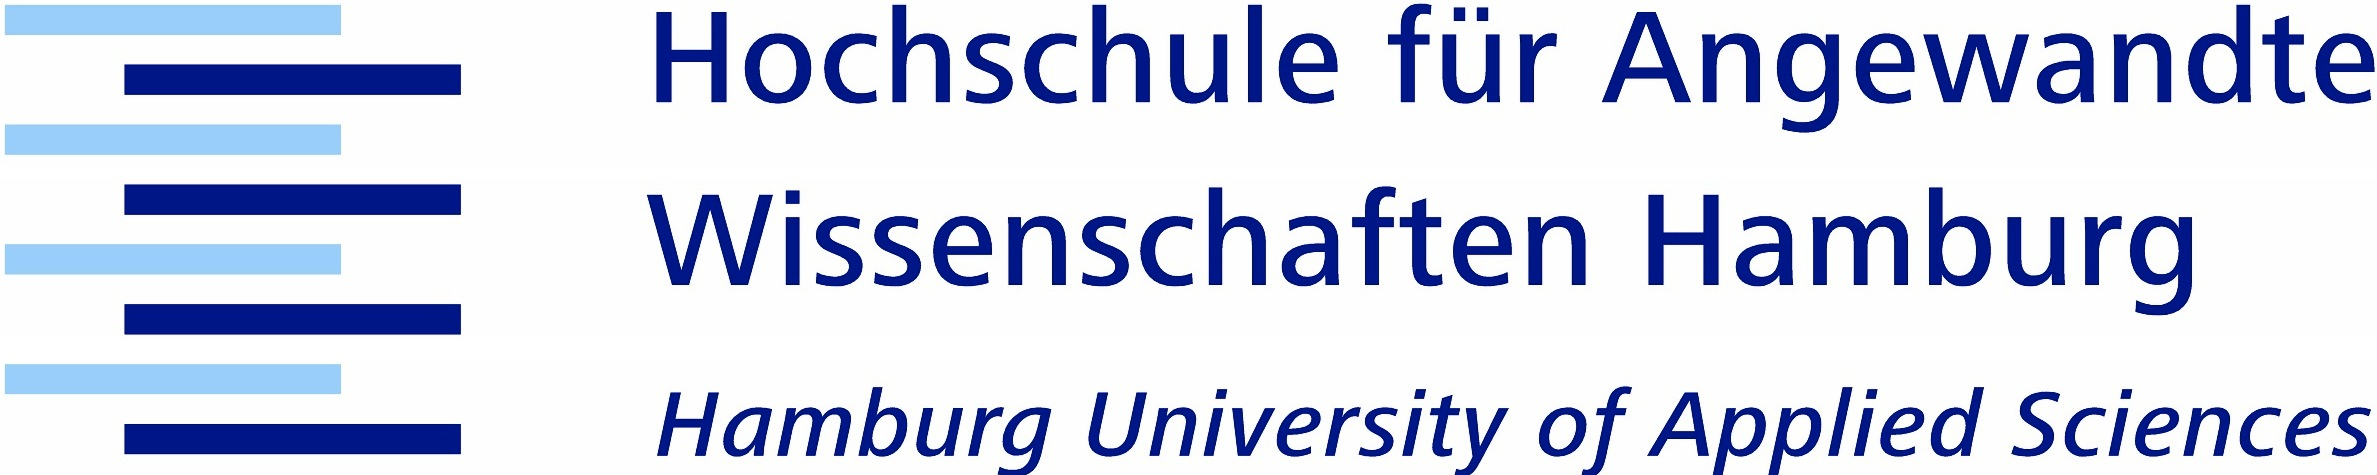
\includegraphics[width=.5\linewidth]{images/hawlogo.png}
  \label{fig:hawlogo}\\
  \small Fakultät Technik und Informatik\\
  \small Department Informations- und Elektrotechnik
  \end{spacing}
  \end{flushright}
\end{figure}
\textbf{\large Bachelorprojekt}
\begin{center}\noindent\textcolor{blue(ncs)}{\rule{13.5cm}{0.5mm}}\end{center}
\begin{spacing}{4.5}
\textbf{\huge Automated Driving}
\end{spacing}
\textbf{\large\indent RC Car Control with Open Source Image Processing}
\begin{center}\noindent\textcolor{blue(ncs)}{\rule{13.5cm}{0.5mm}}\end{center}
\begin{spacing}{1.15}
\vspace*{\fill}
\noindent
\textnormal{\\
  Prof. Dr.-Ing. Marc Hensel \\
  \textbf{Projektgruppe:} Fabian Huber, Enzo Morino, Markus Trockel \\
  \textbf{Abgabe:} DD.MM.2019 \\
}
\end{spacing}
\end{titlepage}
% --- end of titlepage ---

  \pagenumbering{gobble}
  \newpage

  \tableofcontents
  \newpage

  \pagenumbering{arabic}

  \section{Einleitung}
    \ \\

  \section{Ziel des Projekts}
    \ \\
    
    Ziel des Projekts ist es, ein Modell-Auto zu bauen bzw. zu programmieren, das mithilfe eines Raspberry Pi's und einer Kamera autonom zwischen zwei Fahrbahnlinien die Spur halten kann. Das Auto soll auf einer 4 Meter langen geraden Strecke auf der Fahrbahn bleiben, einer Rechts- und einer Linkskurve mit angemessen großem Radius um 90° folgen, und eine Kreisfahrt in beide Richtungen beherrschen können. Optional soll auch eine 8-förmige Strecke wie beim Carolo-Cup befahren werden.
  
  \section{Kurzübersicht}
    \ \\
    
    
  \section{Prinzip der Steuerung}
  	\ \\
  	
  Über ein Python-Programm, welches auf dem Raspberry Pi läuft, wird der Video-Stream der angeschlossenen Kamera iterativ ausgewertet. Es werden die beiden Fahrbahnlinien erkannt, durch Geraden angenähert und deren Fluchtpunkt berechnet. Auf Grundlage der x-Koordinate dieses Fluchtpunktes wird ein Ausgangssignal berechnet, welches über das PWM-Modul den Servo ansteuert, und damit den Lenkwinkel festlegt.  
  	

  \section{Hardware}
    \ \\
    \subsection{Raspberry Pi 3}
    \ \\
    \subsection{Motorcontroller}
    \ \\
    \subsection{Ultraschallsensor}
    \ \\
    \subsection{RC Fahrzeug}
    \ \\
  
  \section{Software}
    \ \\
    \subsection{Aufbau}
    \ \\
    \begin{minipage}{\columnwidth}
      \makeatletter
      \def\@captype{figure}
      \makeatother
      \centering
      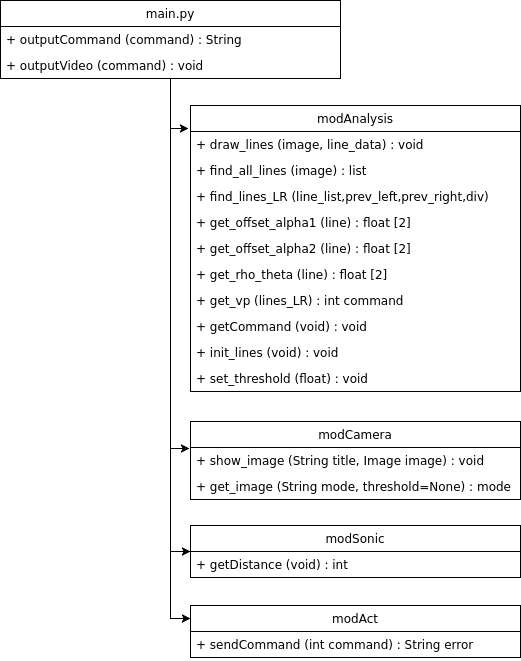
\includegraphics[width=0.8\linewidth]{images/code-flowchart.png}
      \caption{Aufbau des Python Codes}
      \label{fig:image-01}
    \end{minipage}
    \ \\

    \subsection{Externe Module}
    \ \\
    \begin{minipage}{\columnwidth}
      \makeatletter
      \def\@captype{table}
      \makeatother
      \centering
      %\rowcolors{1}{grey}{white}
      \begin{tabular}{ l | l }
      % \multicolumn{2}{|c}{Frame \#} & \multicolumn{4}{|c}{LCD 0/3} &
      Name & Beschreibung \\ \hline \hline
      tkinter & ... \\
      Adafruit\_PCA9685 & Bibliothek zur Ansteuerung des Motorcontrollers \\
      numpy & Bibliothek zur Verwendung von Matlab Funktionen \\
      cv2 & OpenCV 2 bietet Algorithmen zur Bildverarbeitung \\
      io & ... \\
      time & ... \\
      importlib & ... \\
      argparse & ... \\
      pivideostream & ... \\
      picamera & ... \\
      threading & ... \\
      RPi.GPIO & Bibliothek zur Ansteuerung der GPIO ports des Raspbery Pi \\
      \end{tabular}
      \caption{verwendete externe Python Module}
      \label{tab:01}
    \end{minipage}
    
    \subsection{Eigene Module}
    \ \\
    \begin{minipage}{\columnwidth}
      \makeatletter
      \def\@captype{table}
      \makeatother
      \centering
      %\rowcolors{1}{grey}{white}
      \begin{tabular}{ l | l }
      % \multicolumn{2}{|c}{Frame \#} & \multicolumn{4}{|c}{LCD 0/3} &
      Name & Beschreibung \\ \hline \hline
      modAnalysis & Verantwortlich für die eigentliche Verarbeitung der visuellen Informationen \\
      modAct & Verantwortlich für die Ansteuerung des Motors und der Lenkung \\
      modCamera & Bereitet das Kamerabild für die Verarbeitung und Anzeige vor. \\
      modSonic & Kommuniziert mit dem Ultraschallsensor und liefert Distanz zum Hindernis.\\
      \end{tabular}
      \caption{verwendete eigene Python Module}
      \label{tab:01}
    \end{minipage}


      \section{Werkzeuge der Bildverabreitung}
Die folgende Einleitung in die Thematik basiert auf der Lektüre des Buches
"Digitale Bildverarbeitung" von Burger, Burge \citep{burgeDigitBild}, das als 
Literatur für den Einstieg empfohlen wird. Eine zusammenfassende Wiedergabe für 
das Peojekt relevanter Themene ist im Folgenden nachzulesen.\\
Ein Bestandteil der Bildverarbeitung ist die Bildanalyse, bei der es darum geht,
sinnvolle Informationen aus Bildern zu extrahieren. Genauer ist der Bereich der
Computer Vision gefragt, die Sehvorgänge des Menschen in der dreidimensionalen Welt
zu mechanisieren.\\
Die Steuerung des Wagens soll durch Informationen aus den Kamerabildern
erfolgen: Durch Erkennen der Fahrbanhlinien soll die Lenkung innerhalb der Spur
geregelt werden.\\
Dieser Prozess lässt sich beschreiben mit:
\begin{enumerate}
  \item Digitalisierung mit Hilfe der Kamera
  \item Vorverarbeitung (Bildverbesserung bzw. Anpassung an den Zweck) durch
    Umwandlung in ein binäres Canny-Edges-Bild
  \item Segmentierung eine Vorauswahl des Bildauschnittes mit den relevante
    Informationen
  \item Merkmalsextraktion zur Linienerkennung durch die Hough-Transformation
  \item Parametrisierung als mathematische  Beschreibung der Fahrbahnlinien zur
    weiteren Informationsverarbeitung
\end{enumerate}

\subsection{Digitalisierung}
Der von der Kamera aufgenommen Bilder-Stream liegt in digitaler Form vor. Dabei lassen
sich benötigte Parameter eintellen(ergänzen Fabian?). Um ein optimales Bild zu
erhalten sind die Beleuchtungsumstände zu beachten, da hierdurch die
Differenzierung von Linien im Bild beeinflusst wird. Beachte timing? \\
In der Bildverabreitung ist der Nullpunkt der x- und y-Achse in der linken
oberen Ecke des Bildes definiert, was für ein eindeutiges Anwenden von Prozessen
und daraus generierten Informationen relevant ist.

\subsection{Vorverarbeitung- Canny-Kantenoperator}
Zur späteren Erkennung der Linien werden die dafür relevanten Informationen aus
dem Bild gefiltert: sogenannte Bildkannten. Bildkanten sind Übergangsstellen, wo
ein hoher Grauwertsprung von einem Pixel zum Nachbarpixeel erfolgt, wie z. B. bei 
einem weißen Farbahnstreifen zwei Kannten erkannt werden sollen.\\
Die Canny-Edges-Funktion aus der openCV Library ist ein bewährter Algorithmus zur Kantenerkennung, da drei Ziel
gleichzeitig erreicht werden drei Zile: ein zuverlässiges Detektieren
vorhandener Kanten, die Position der Kante präzise zu bestimmen, und Farbsprünge, 
die nicht als Kante interoretiert werden sollen, auszulassen.\\

\subsection{Segmentierung}
[BILD Kamera mit Fahrbahnlinien]
Der für die Erkennung der Fahrbahnlinien relevante Bereich liegt in einem
unteren Dreieck des Kamerabildes. Dieser Teil wird ausgewählt, bzw. davon ausserhalb
liegende Bereiche werden nicht bei der Erkennenung der Farbahnlinien
berücksichtigt.\\

\subsection{Merkmalsextraktion zur Linienerkennung}
Das Canny-Kantenbild wird mit Hilfe der Hough-Transformation aus der
openCV-Library in den Hough-Raum transformiert, wo dann die Erkennung der Linien
erfolgt.

\begin{minipage}{\columnwidth}
  \makeatletter
  \def\@captype{figure}
  \makeatother
  \centering
  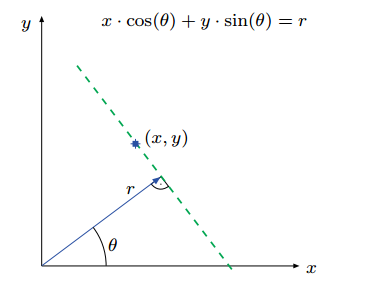
\includegraphics[width=0.8\linewidth]{images/gradeThetaR.png}
  \caption{gradeThetaR.png}
  \label{fig:gradeThetaR}
\end{minipage}

Dabei kommt zur Anwendung, dass eine Gerade mathematisch sowohl mit $y
= m \dot x + b$ als auch mit $r(\theta) = x \cdot cos(\theta) + y \cdot
sin(\theta)$ beschrieben werden kann. Dabei ist in der zweiten Beschreibung 
$\theta$ der  Winkel des Radius $r$ zum Urspung, an dessen Ende senkrecht die
beschriebene Grade verläuft. Zu Bedenken ist, dass wie schon erwähnt der
Koordinatenursprung des Bildes oben links definiert ist.\\
Das rechenaufwendige Verfahren der Hough-Transformation generiert für jeden
Kantenbildpunkt des Canny-Edges-Bildes Bildpunkte im Hough-Raum, dessen Achsen
ein $\theta$ / $r$ - Koordinatensystem bilden. Linien im kartesisches System
sind als Punkthäufungen im Hough-Raum erkennbar. Liegt eine Anzahl von
Punkten oberhalb eines zu definierenden Schwellwertes, wird eine Linie erkannt
und die Houh-Transformationsfunktion gibt ein Wertpaar $\theta$, $r$ zurück.




	\section{Iterative Auswertung des Kamerabildes}	

	Das Bild der Kamera werden iterativ ausgewertet um die beiden Fahrbahnlinien zu erkennen und daraus ein Ausgangssignal für die Steuerung zu generieren. Der gewählte Ansatz war es, die Fahrbahnlinien durch zwei Geraden anzunähern. Die Funktion HoughLines wird verwendet um die Fahrbahnlinien zu erkennen und die zugehörigen Geraden zu berechnen. Da die Funktion HoughLines in den meisten Fällen nicht nur die beiden Fahrbahnlinien erkennt, sondern alle möglichen Geraden, bestand die erste Aufgabe darin, nur die Geraden herauszufiltern, welche die Fahrbahnlinien repräsentieren, und alle anderen Geraden zu verwerfen. Im Programm wird dies erreicht, indem alle Geraden, die durch die Funktion HoughLines gefunden wurden mit dem Geradenpaar aus dem vorherigen Programmdurchlauf verglichen werden, und nur ähnliche Geraden beibehalten werden.\\
	
	Beim Start des Programm werden für die beiden Geraden feste Werte vorgegeben, die dann korrigiert und an die erkannten Linien angepasst werden. In Abbildung \ref{fig:fahrbahn} ist dies bildlich dargestellt. Die roten Linien sind zu Beginn des Programms fest vorgegeben. Die blauen Linien sind das Ergebnis der Korrektur durch das Programm.
	
	\begin{figure}[H]
		\centering
		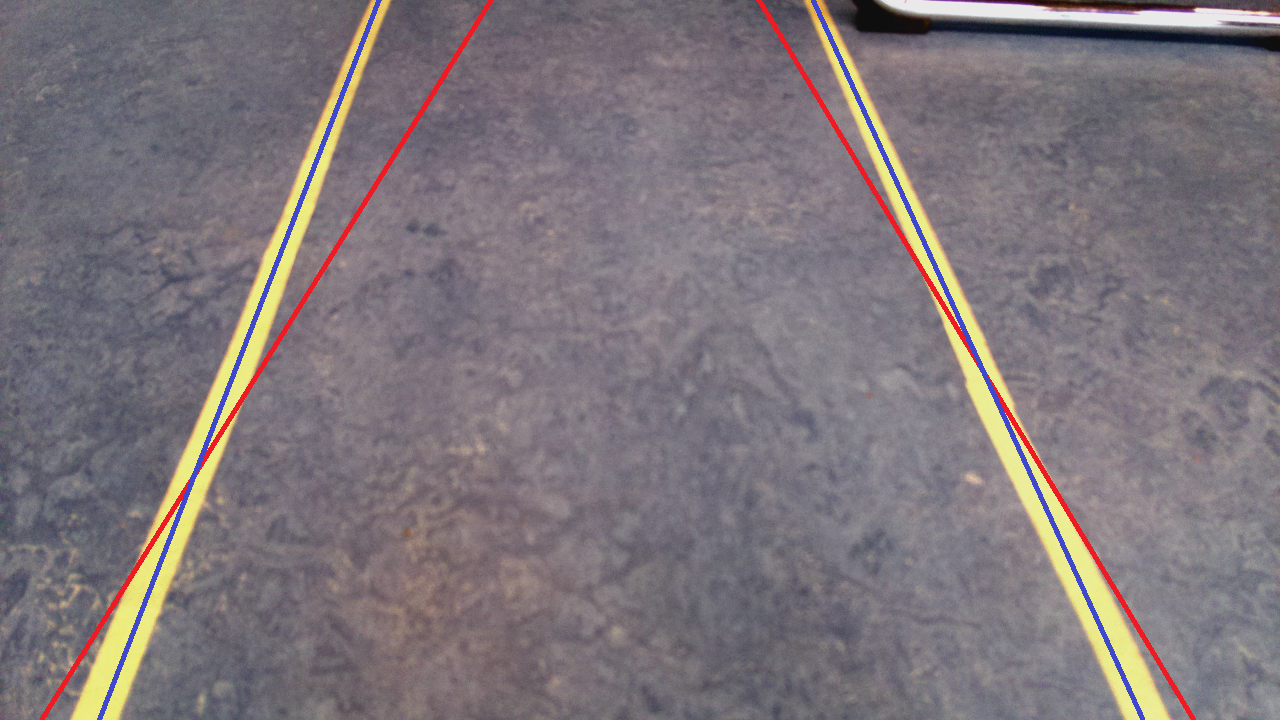
\includegraphics[width=.5\linewidth]{images/fahrbahn.png}
		\caption{Beispiel für die erste Form der Geradenrepräsentation}
		\label{fig:fahrbahn}
	\end{figure}
	
	
	Der Vergleich der Geraden wird durchgeführt, indem um die beiden Geraden aus dem letzten Durchlauf ein Toleranz-Fenster gelegt wird, und von allen gefundenen Geraden nur diejenigen herausgefiltert werden, die innerhalb dieses Toleranz-Fensters liegen. Von diesen Geraden wird dann der Durschnitt berechnet, sodass nur noch zwei Geraden für die beiden Fahrbahnlinien übrig bleiben. \\
	
	Eine Schwierigkeit besteht darin die Geraden so zu repräsentieren, dass diese gut miteinander vergleichbar sind. Bei einer geringen Änderung einer Geraden von einem zum nächsten Zyklus sollen sich deren Parameter dabei auch nur geringfügig ändern. Ansonsten werden ähnliche Geraden beim filtern verworfen, da deren Parameter nicht im Toleranzfenster liegen. Im Programm wurden daher je nach Anwendungsfall verschiedene Repräsentationsformen verwendet, welche im folgenden beschrieben werden.
	
	\subsection{Verwendete Repräsentationsformen von Geraden}
	
	Als erstes wurde die $\rho$-$\theta$-Form verwendet (der Name ist frei gewählt). Dies ist die Form, die von der Funktion HoughLines verwendet wird. Sie besteht aus einem Radius $\rho$ und einem Winkel $\theta$. $\theta$ ist der Winkel zwischen der Normalen, die senkrecht auf der Geraden steht, und der x-Achse. Der Winkel  $\rho$ ist die Länge dieser Normalen, d.h. der Abstand zwischen der Geraden und dem Ursprung des Koordinatensystems. Der Winkel 
	Abbildung \ref{fig:rho_theta1} zeigt ein Beispiel für die Repräsentation zweier Fahrbahnlinien in der $\rho$-$\theta$-Darstellung, für den Fall, dass der Wagen relativ mittig und gerade auf der Fahrbahn steht. Das Rechteck symbolisiert die Ränder des Kamerabildes. Der Koordinatenursprung liegt in der oberen linken Ecke. $\theta1$ ist positiv, $\theta2$ negativ. $\rho1$ und $\rho2$ sind jeweils die Abstände der Geraden vom Koordinatenursprung.
	
	\begin{figure}[H]
		\centering
		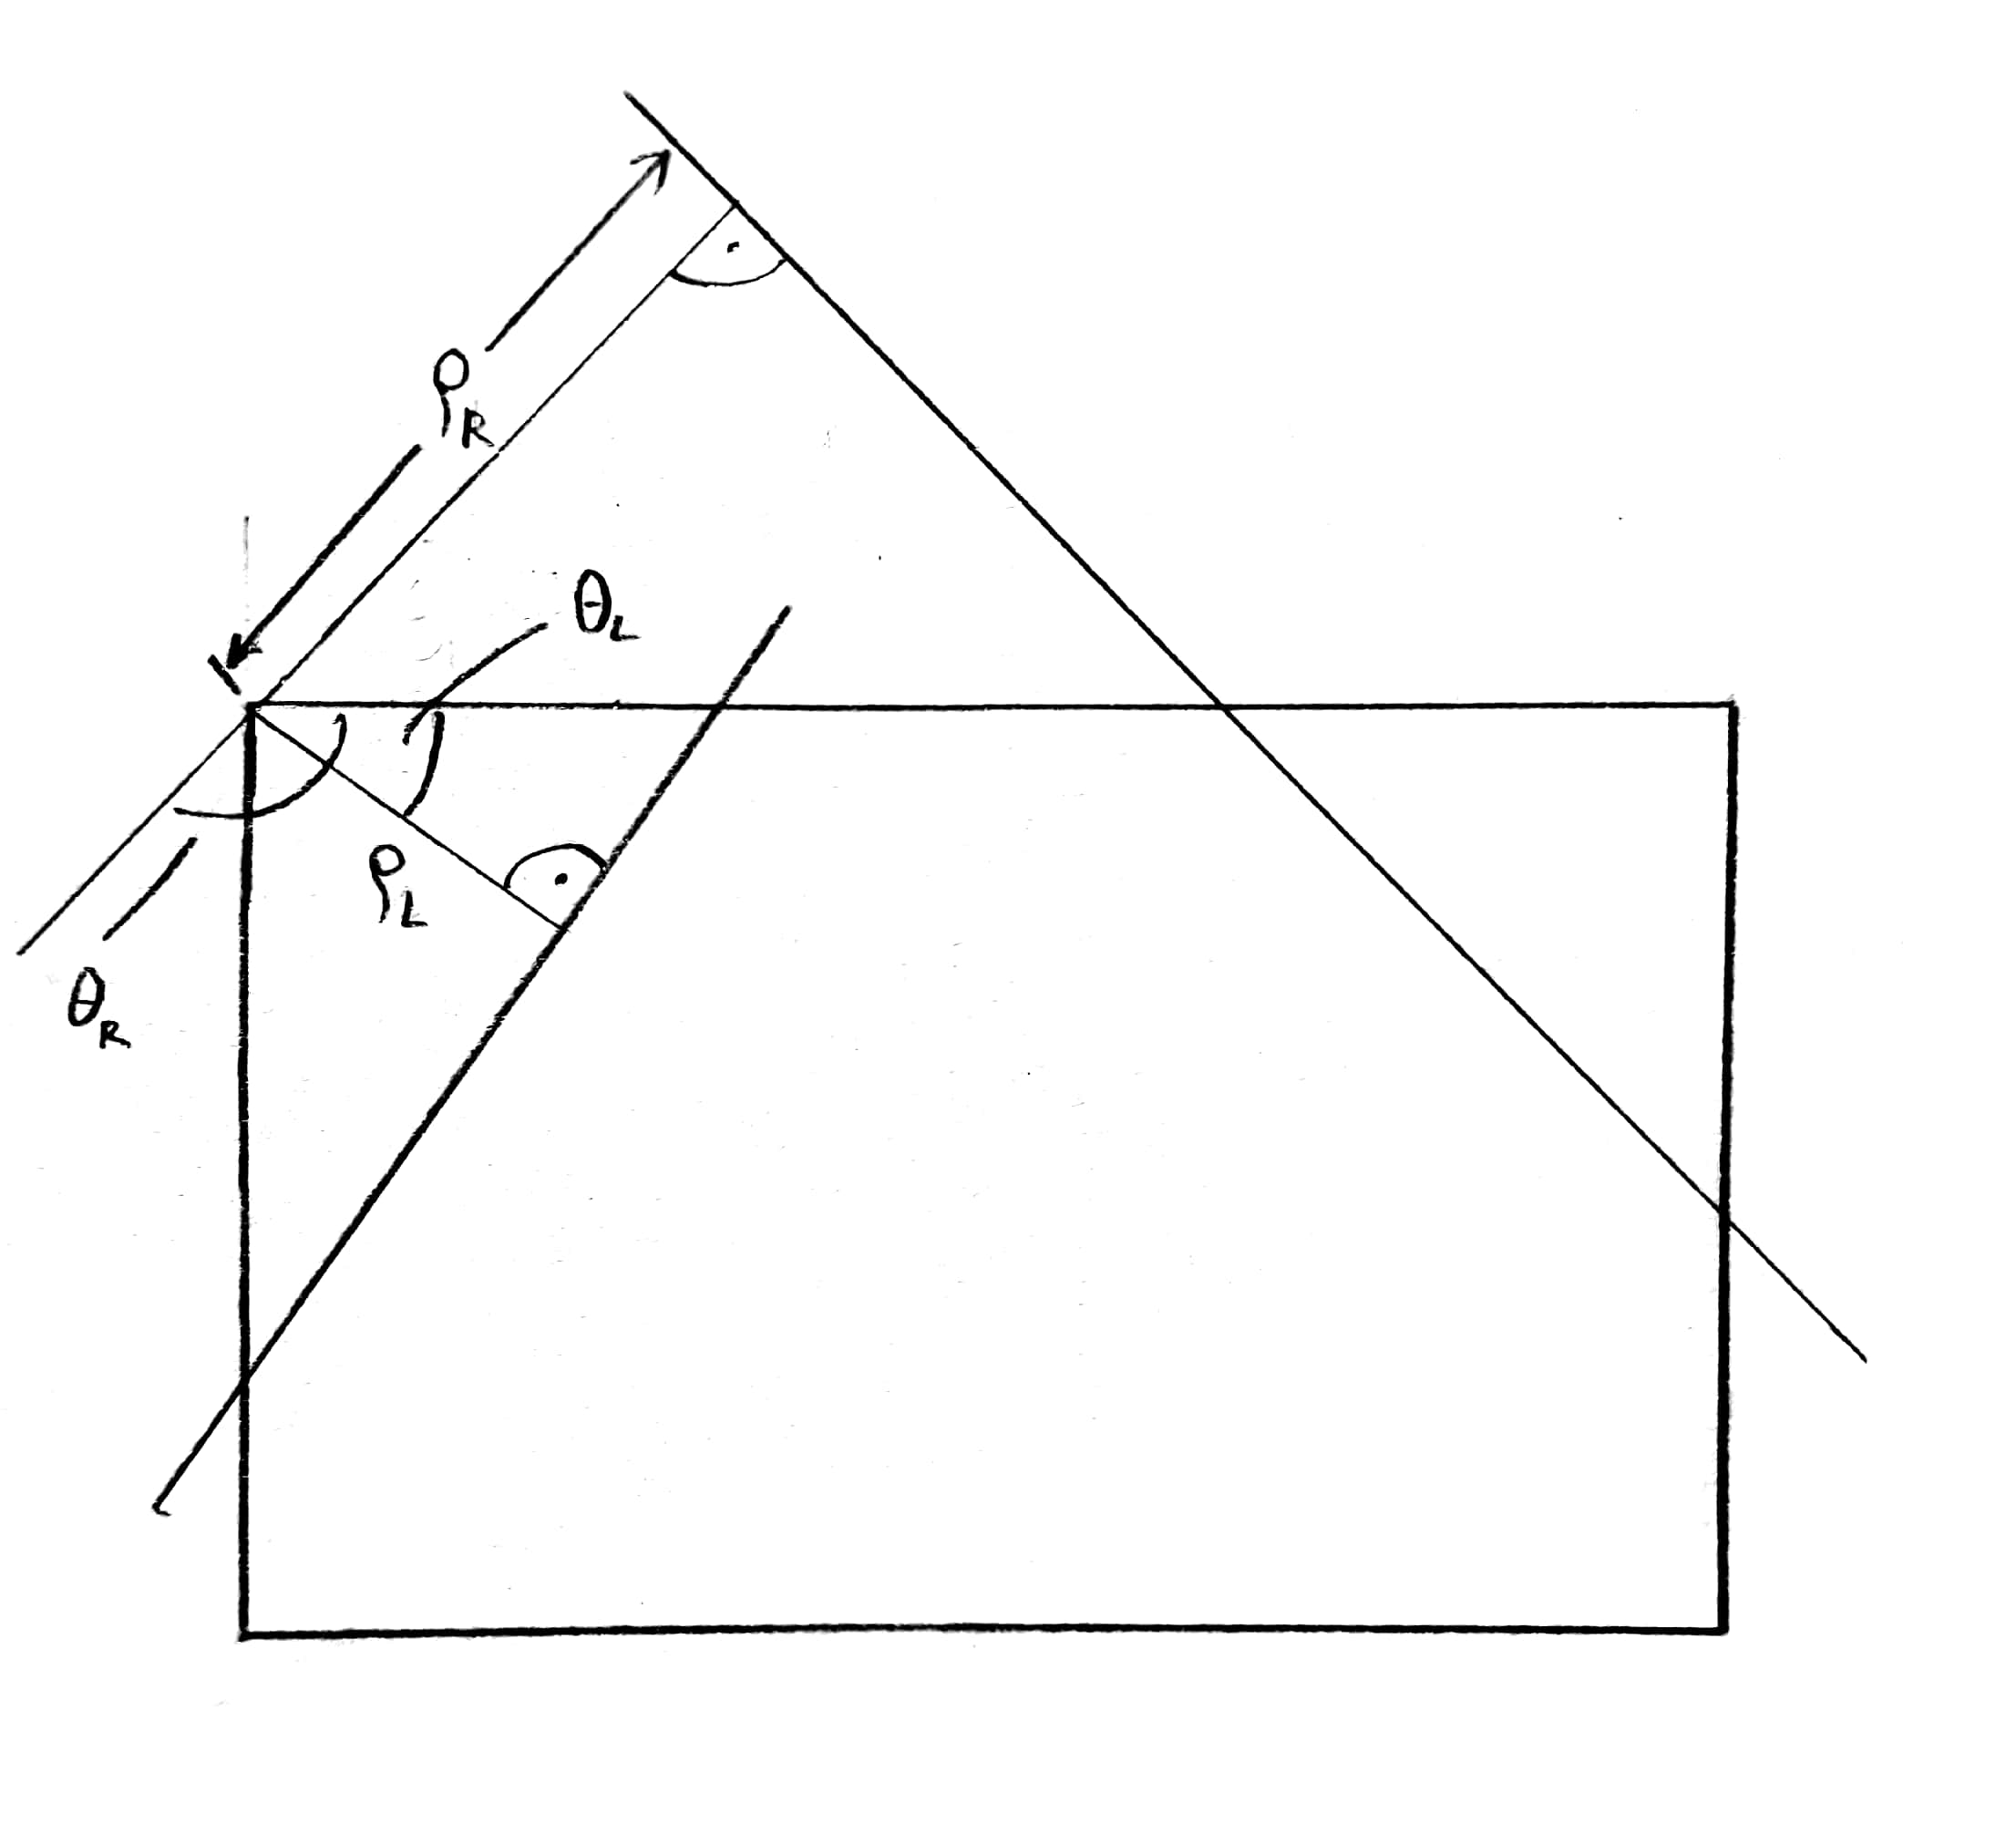
\includegraphics[width=.5\linewidth]{images/rho_theta1.jpg}
		\caption{Beispiel für die erste Form der Geradenrepräsentation}
		\label{fig:rho_theta1}
	\end{figure}
	
	Eine Schwäche dieser Repräsentationsform wird liegt darin, dass zwei sehr ähnliche Geraden komplett verschiedene Winkel $\theta$ haben können. Dies wird in Abbildung \ref{fig:rho_theta2} deutlich. $\theta1$ beträgt hier ca. $70^\circ$, $\theta2$ ca. $-100^\circ$.
	
	
	
	\begin{figure}[H]
		\centering
		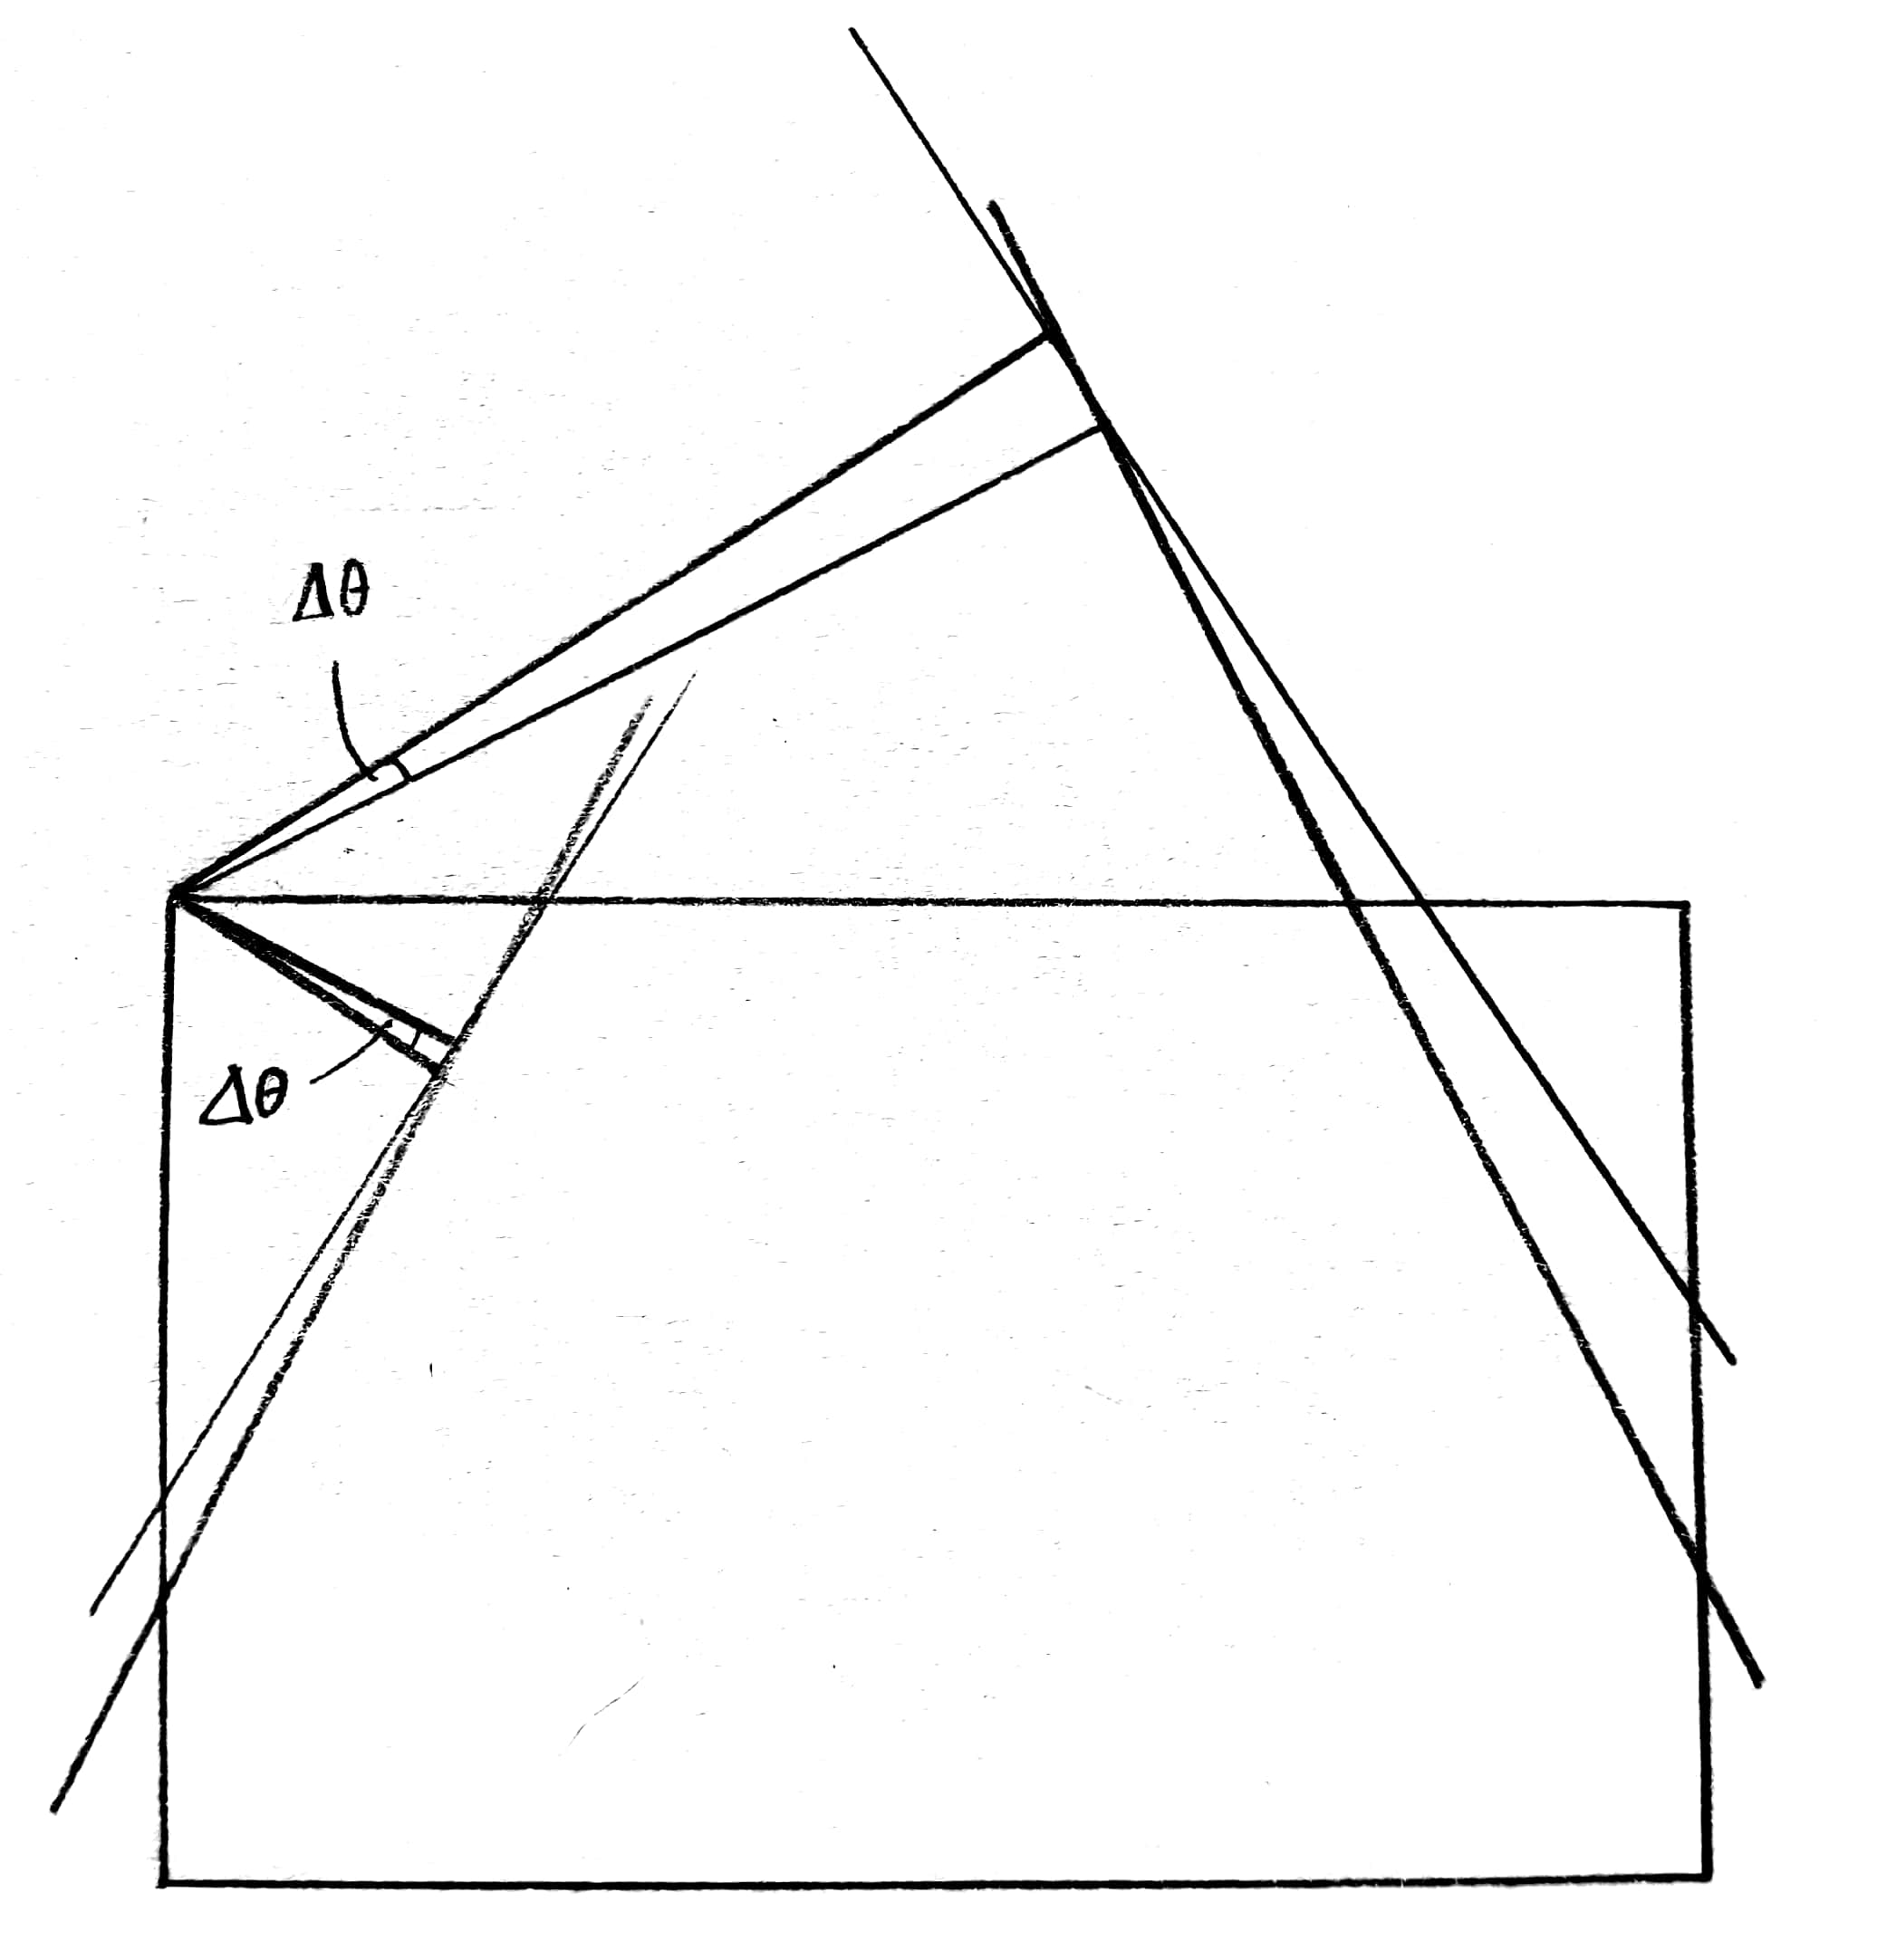
\includegraphics[width=.5\linewidth]{images/rho_theta2.jpg}
		\caption{Beispiel für die erste Form der Geradenrepräsentation}
		\label{fig:rho_theta2}
	\end{figure}

	Um dieses Problem zu umgehen wurden die Geraden mithilfe der Funktion offset\_alpha1 in eine andere Form umgerechnet, bei der diese durch den Offset $\omega$ auf der y-Achse und den Winkel zur x-Achse beschrieben werden. Die Umrechnung erfolgt folgendermaßen:\\
	
	Für Winkel $\theta<90^\circ$:
	
	\begin{align*}
		\omega&=-\frac{\rho}{\cos{90^{\circ}-\theta}} \\
		\alpha&=90^{\circ}-\theta
	\end{align*}
	
	Für Winkel $\theta>90^\circ$:
	
	\begin{align*}
		\omega&=-\frac{\rho}{\cos{\theta-90^{\circ}}} \\
		\alpha&=\theta-90^{\circ}
	\end{align*}
	
	Abbildung \ref{fig:alpha_omega1} veranschaulicht die Repräsentation der beiden Fahrbahnlinien in dieser Form.
	
	\begin{figure}[H]
		\centering
		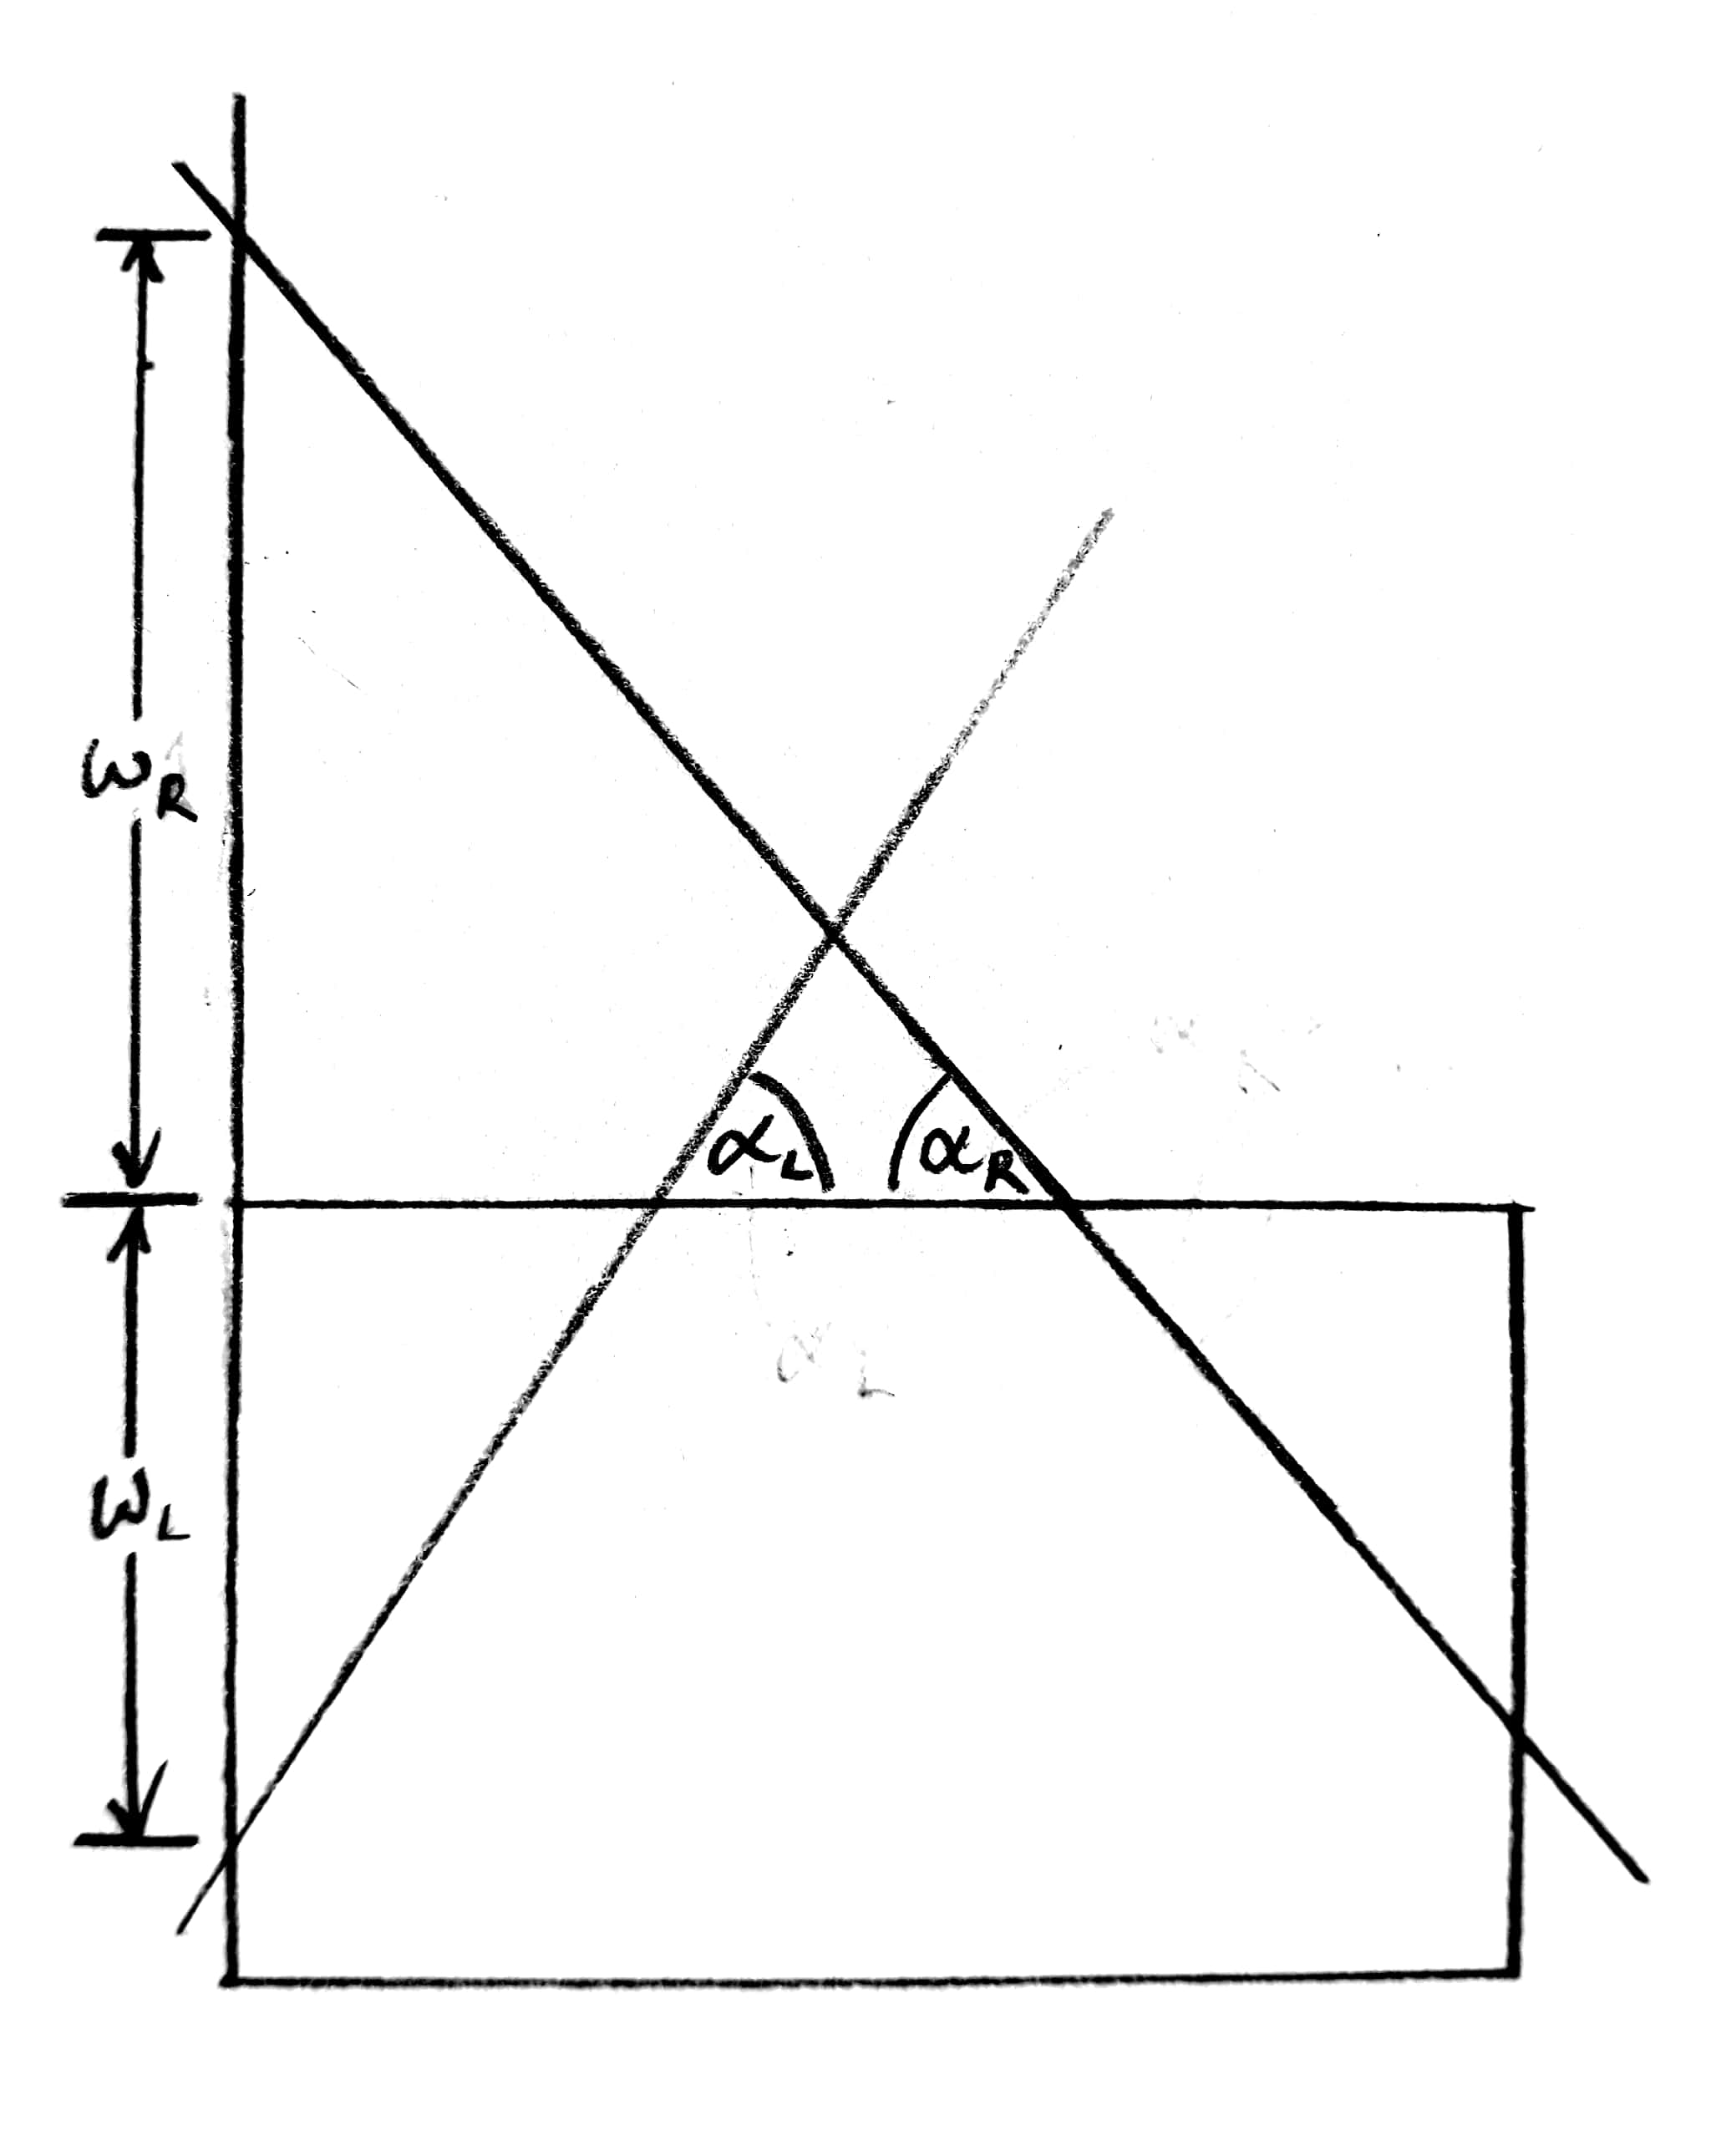
\includegraphics[width=.5\linewidth]{images/alpha_omega1.jpg}
		\caption{Beispiel für die erste Form der Geradenrepräsentation}
		\label{fig:alpha_omega1}
	\end{figure}

	Auch bei dieser Form ergibt sich das Problem, dass sich bei geringfügiger Veränderung der Geraden deren Parameter in bestimmten Situationen stark ändern. Dies ist besonders für die rechte Fahrbahnlinie der Fall, wie sich in Abbildung \ref{fig:alpha_omega2} erkennen lässt. Hier sieht man, dass sich der Offset $\omega$ stark ändert, wenn sich der Winkel der Geraden leicht ändert.


	\begin{figure}[H]
		\centering
		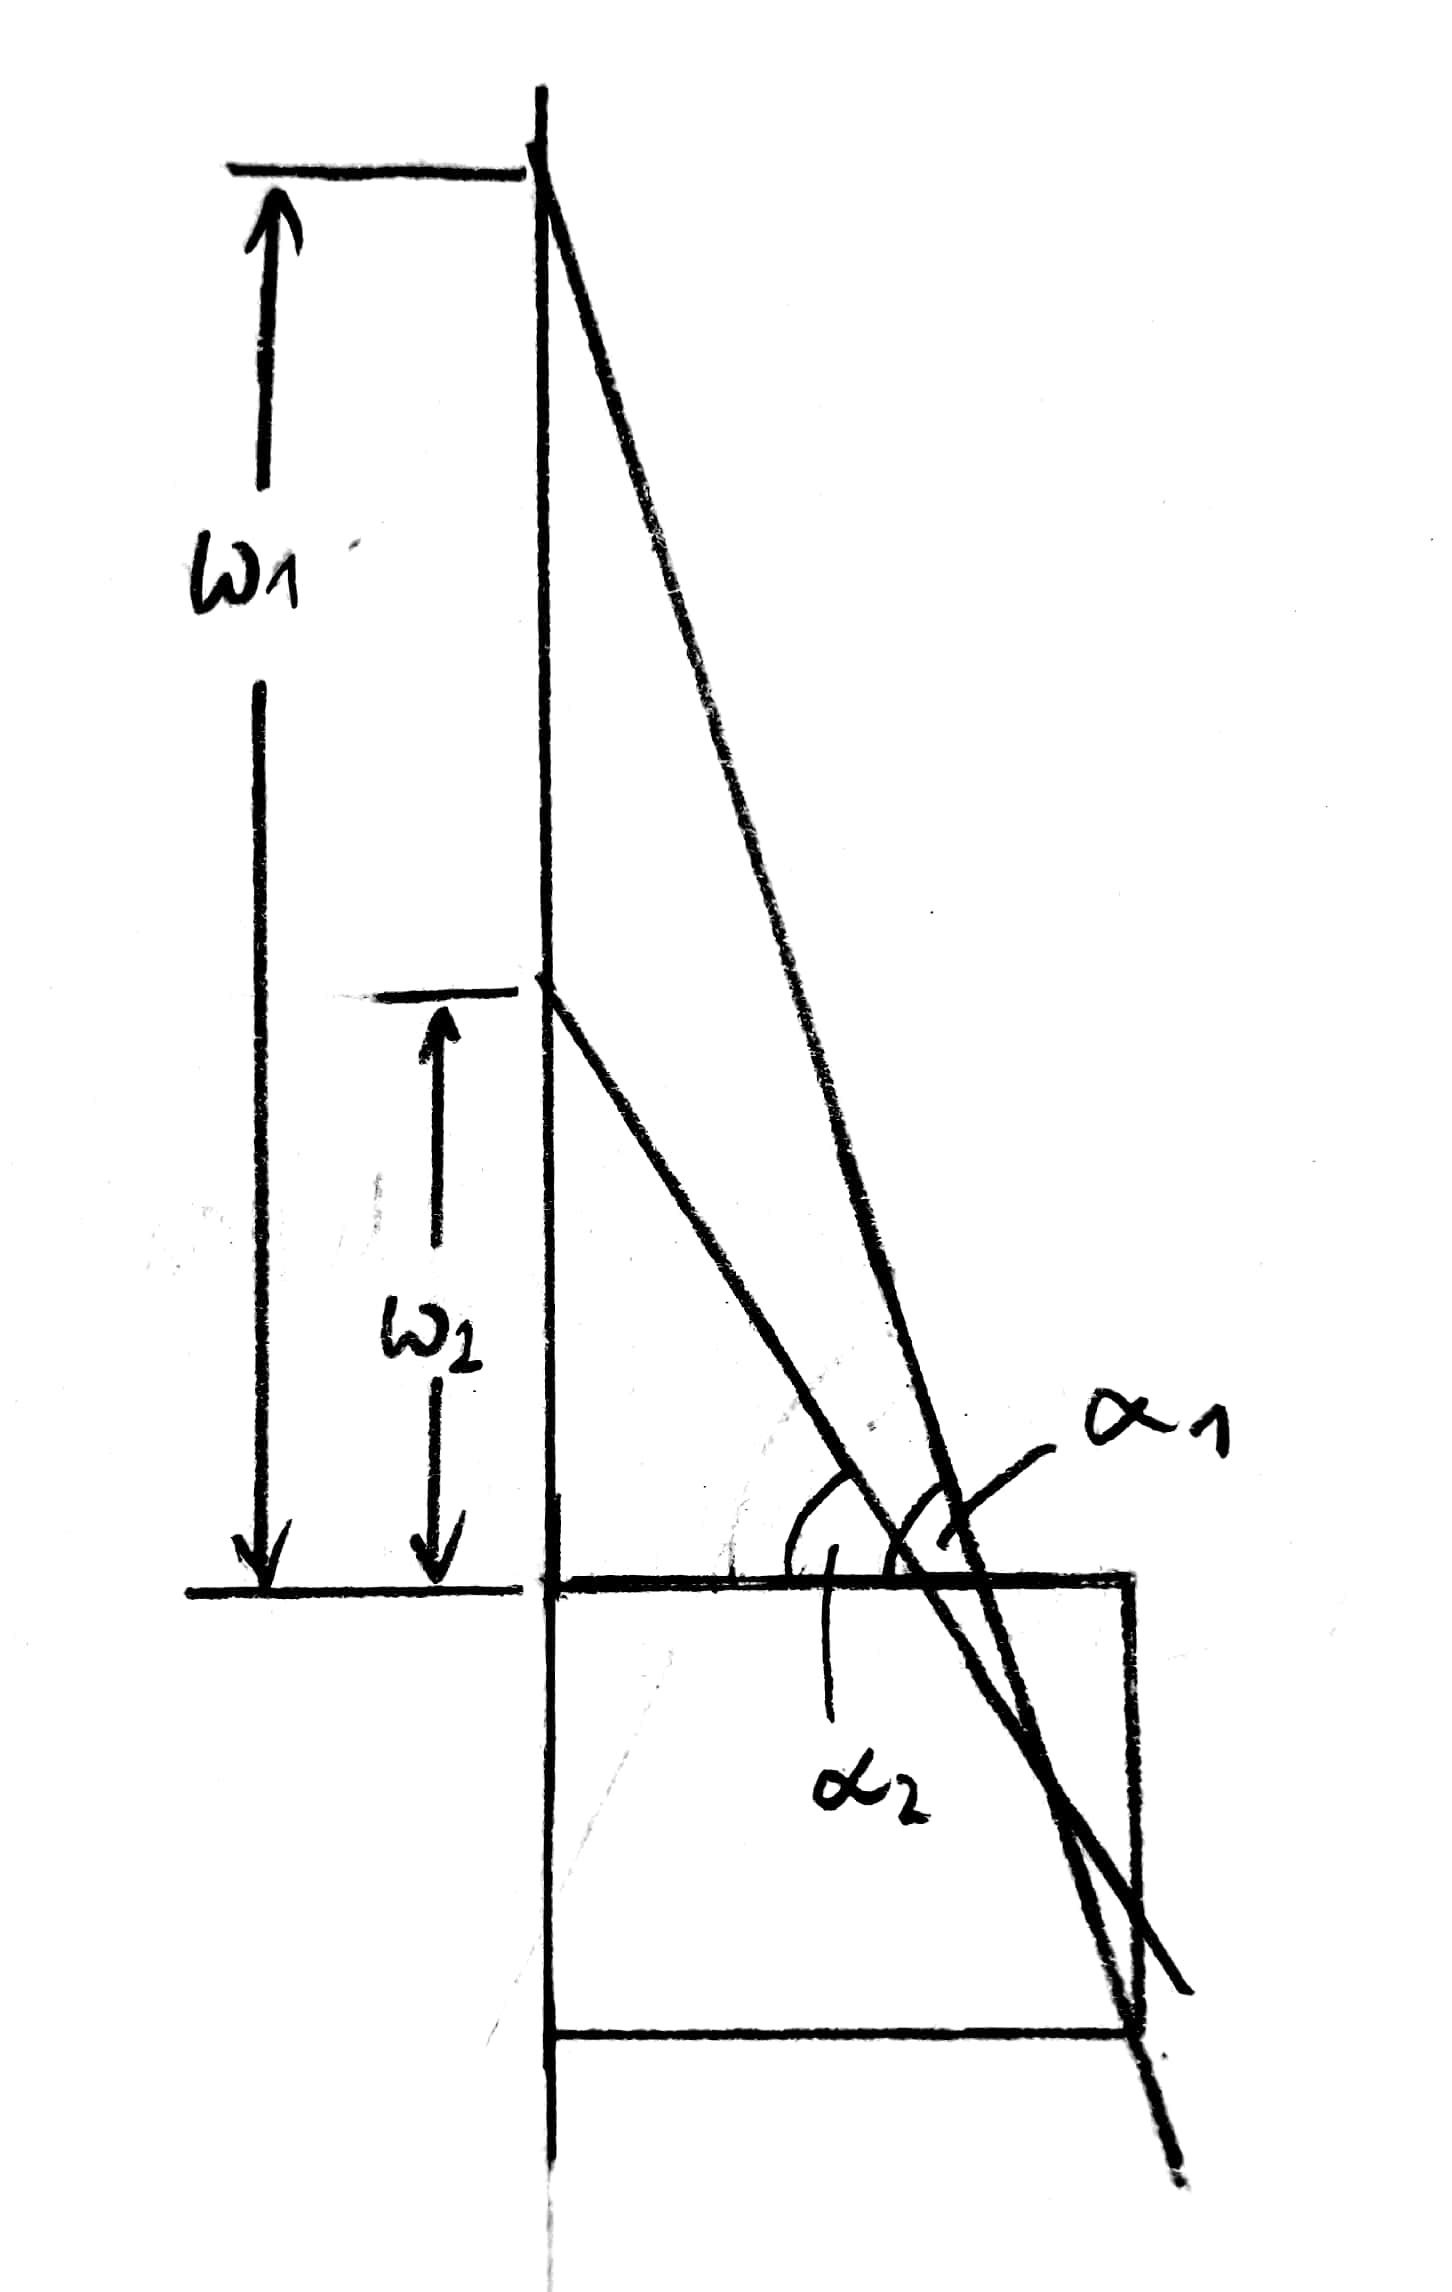
\includegraphics[width=.3\linewidth]{images/alpha_omega2.jpg}
		\caption{Beispiel für die erste Form der Geradenrepräsentation}
		\label{fig:alpha_omega2}
	\end{figure}
	
	
	
	
	
%	Beim Start des Programms werden für die beiden Geraden feste Werte vorgegeben. Anhand dieser Anfangswerte werden die im nächsten Durchlauf die Fahrbahnlinien durch bessere Werte angenähert.\\
%	Dafür wird das Bild zunächst mithilfe eines Schwellwertes in Schwarzweiß umgewandelt. Bei einem geeigneten Schwellwert sollten nun möglichst nur die beiden Fahrbahnlinien weiß sein (den Wert 1 haben).\\
%	Als nächstes wird die Funktion HoughLines aus der Bibliothek cv ausgeführt, die alle Geraden im Bild sucht. Die Funktion Houghlines gibt als Rückgabewert eine Liste von Geraden zurück, die in Polarkoordinaten durch einen Winkel $\rho$ und ein Abstand $\theta$ repräsentiert werden. $\rho$ ist der Winkel zwischen der Normalen, die senkrecht auf der Geraden steht, und der x-Achse. $\theta$ ist die Länge dieser Normalen, d.h. der Abstand zwischen der Geraden und dem Ursprung des Koordinatensystems.
	
 
	
	

  % \bibliography{hawey-documentation}
  % \bibliographystyle{ieeetr}

      % Bibliograpy / Literaturverzeichnis
      \newpage
      \addcontentsline{toc}{section}{Literaturverzeichnis}
      % displsy bibliography
      \bibliography{bibliography}

\end{document}
